\documentclass[a4paper,twoside]{article}
\usepackage[T2A]{fontenc}
\usepackage[utf8x]{inputenc}
\usepackage{amssymb}
\usepackage{amsmath}
\usepackage{amsthm}
\usepackage{latexsym}
\usepackage{indentfirst}
\usepackage{bm}
\usepackage{enumerate}
\usepackage{graphicx}
\usepackage{epsf}
%\usepackage{epsfig}
%\DeclareGraphicsExtensions{.pdf,.png,.jpg}
\usepackage{wrapfig}
\usepackage{euscript}
\usepackage{indentfirst}
\usepackage[russian]{babel}
\usepackage{minted}
\usepackage{pgfplots}

\graphicspath{{figures/}}

\sloppy\unitlength=.24mm
\renewcommand{\thefootnote}{\arabic{footnote}}

\textwidth=132mm
\headheight=7mm
\headsep=5mm
\textheight=200mm
\oddsidemargin=0mm
\evensidemargin=0mm
\topmargin=0mm

\newcommand{\firstheader}[1]{\noindent\textbf{#1}\nopagebreak\bigskip}
\newcommand{\header}[1]{\bigskip\medskip\noindent\textbf{#1}\nopagebreak\bigskip}
\newcommand{\subheader}[1]{\bigskip\medskip\noindent\emph{#1}\nopagebreak\bigskip}
\newcommand{\subsub}[1]{\bigskip\medskip\noindent\emph{#1}\nopagebreak\bigskip}

\theoremstyle{theorem}
\newtheorem{theorem}{Теорема}
\newtheorem{Theorem}{Теорема}
\newtheorem{definition}{Определение}
\newtheorem{Def}{Определение}
\newtheorem{corollary}{Следствие}
\newtheorem{proposition}{Предложение}
\newtheorem{prop}{Предположение}
\newtheorem{lemma}{Лемма}
\newtheorem{assumption}{Предположение}
\newtheorem{Lemma}{Лемма}
\newtheorem{Cons}{Следствие}
\newtheorem{Proposition}{Предложение}
\newtheorem{Statement}{Утверждение}
\newtheorem{statement}{Утверждение}
\theoremstyle{remark}
\newtheorem{remark}{Замечание}
\newtheorem{Remark}{Замечание}
\newtheorem{example}{Пример}
\newtheorem{Example}{Пример}
\newtheorem{notation}{Замечание}
\newtheorem{teo}{Теорема}
\newtheorem{sled}{Следствие}
\newtheorem{sublemma}[theorem]{\indent\bf Подлемма}
\newtheorem{problem}{\indent\bf Проблема}
\newtheorem{hypothesis}{\indent\bf Гипотеза}
\newtheorem{denotation}[theorem]{\indent\bf Обозначение}
\newtheorem{thr}{Теорема}
\newtheorem{crl}[thr]{Следствие}
\newtheorem{lmm}[thr]{Лемма}
\newtheorem{qu}{Вопрос}
\newtheorem{dfn}{Определение}
\newtheorem{approval}{Утверждение}

% нумерацию можно оставить как есть
\newcommand{\pages}{1-8}

\begin{document}
\pagestyle{headings}
\makeatletter
%\renewcommand{\@evenhead}{\raisebox{0pt}[\headheight][0pt]{\vbox{\hbox to\textwidth{\thepage\hfill \strut {\small БЕНИНГ В.Е., САВУШКИН В.А.}}\hrule}}}
%\renewcommand{\@oddhead}{\raisebox{0pt}[\headheight][0pt]{\vbox{\hbox to\textwidth{{\small О ДЕФЕКТЕ ВЫБОРОЧНОЙ МЕДИАНЫ В СЛУЧАЕ ВЫБОРОК... }\hfill \strut\thepage}\hrule}}}
%\makeatother

%%%%%%%%%%%%%%%%%%%%%%%%%%%%%%%%%%%%%%%%%%%%%%%%%%%%%%%%%%%%%%%%%%%%%%%%%%%%%%%%%%%%%%%%%%%%%%%%%%%%%%%%
% Заголовок
%%%%%%%%%%%%%%%%%%%%%%%%%%%%%%%%%%%%%%%%%%%%%%%%%%%%%%%%%%%%%%%%%%%%%%%%%%%%%%%%%%%%%%%%%%%%%%%%%%%%%%%%
%\thispagestyle{plain}
%УДК 510.676, 519.7
\begin{center}
{\bf Сравнение возможностей логистической регрессии и искусственных нейронных сетей в прогнозировании результатов исследования на малой выборке}
\vspace{4mm}\par
{\bf Базылев В.В.$^{*}$, Карнахин В.А.$^{*}$}\\
$^{*}$Федеральный центр сердечно-сосудистой хирургии \\ 
Министерства здравоохранения России\\
\end{center}
\vspace{2mm}\par

\begin{quote}
В работе доказаны теоремы, позволяющие находить асимптотический дефект выборочной медианы, основанной на выборках случайного объема. Это делает возможным сравнивать в терминах добавочного числа наблюдений качество выборочной медианы, основанной на выборках случайного и неслучайного объемов. Рассмотрены случаи биномиального и распределения Пуассона.
\end{quote}

\begin{quote}
{\bf Ключевые слова:} искусственные нейронные сети, логистическая регрессия, статистика,
выборка, математическая модель, регрессия.
\end{quote}



%%%%%%%%%%%%%%%%%%%%%%%%%%%%%%%%%%%%%%%%%%%%%%%%%%%%%%%%%%%%%%%%%%%%%%%%%%%%%%%%%%%%%%%%%%%%%%%%%%%%%%%%
% Статья
%%%%%%%%%%%%%%%%%%%%%%%%%%%%%%%%%%%%%%%%%%%%%%%%%%%%%%%%%%%%%%%%%%%%%%%%%%%%%%%%%%%%%%%%%%%%%%%%%%%%%%%%

\firstheader{Введение}

Прогностические модели искусственных нейронных сетей (ИНС) и логистической регрессии используются в различных областях медицины для решения различных задач (Han, 2018; García-Reiriz, 2007; Bhatikar, 2005; Zhang, 1998; Waisman, 2019; Cireşan, 2012; Parisi, 2019). ИНС, создание которых было вдохновлено нейробиологией и архитектурой человеческого мозга являются непараметрическими методами распознавания образов, которые выявляют скрытые связи между зависимыми и независимыми переменными (Haykin, 1999; Lobo, 2018; Bazrafkan, 2018; Plis, 2018; Soltoggio, 2018; Parisi, 2019; Vellappally, 2019; Hyvärinen, 2000). В последние годы нейронные сети получили широкое распространение во многих дисциплинах науки и медицины. Модели нейронных сетей могут учиться на примерах, включать большое количество переменных и предоставлять адекватный и быстрый ответ на новые входящие данные (Tavanaei, 2019; Kulkarni, 2018; Graves, 2005; Boutin, 2018; Zhang, 2018; Coninck, 2018; Wideman, 2018). В настоящее время все чаще предпринимаются попытки сравнивать различные количественные модели для решения конкретных задач классификации данных (Sargent, 2001; Dreiseitl, 2002; Zurada, 1994). D.J. Sargent (Sargent, 2001) представил метаанализ, сравнив ИНС с регрессионными моделями в 28 исследованиях и обнаружил, что в 36\% случаев ИНС оказались более эффективны, чем регрессионные модели. Логистическая регрессия обладала преимуществом в 14\% работ, в оставшихся 50\% исследований производительность моделей была одинаковой. S. Dreiseitl (Dreiseitl, 2002) проанализировал 72 статьи, сравнивая ИНС с логистической регрессией и обнаружил преимущество нейронных сетей в 18\% случаев, а логистической регрессии только в 1\%, в 42\% случаев не было никакой разницы между двумя моделями. При этом в литературе отсутствуют данные о сравнении математических моделей в условиях малых выборок и сложных клинических ситуаций. Для ответа на вопрос о преимуществе в прогнозировании результатов работы при малых выборках выполнено симуляционное исследование.

Цель работы: cравнить производительность моделей ИНC и логистической регрессии в прогнозировании результатов исследования в условиях малой выборки.

\header{Материалы и методы}

\textbf{Логистическая регрессия}

Логистическая регрессия — это статистическая модель, используемая для предсказания вероятности возникновения некоторого события путём подгонки данных к логистической кривой. Методика используется для определения предсказания вероятности возникновения некоторого события по значениям множества признаков.
Логарифм правдоподобия логистической регрессии имеет вид:

\begin{equation}
	L(\beta) = \sum_{i=1}^{n}\left(l_i(\beta)\right)
\end{equation}

где, $\beta$ - вектор параметров.

Обучение логистической рагрессии на языке Python и библиотеки scikit-learn:

\begin{minted}{python}
	# 1. Обучение логистической регрессии
	logreg = LogisticRegression(max_iter=1000)
	logreg.fit(x_train, y_train)
	
	# 2. Вывод весовых коэффициентов
	print("Весовые коэффициенты модели:")
	print(pd.DataFrame({'feature': x_train.columns, 'coef': logreg.coef_[0]}))
	
	# 3. Вывод значений, возвращаемых моделью (степень уверенности)
	# для первых 10 примеров
	probabilities = logreg.predict_proba(x_train[:10])
	print("\nСтепень уверенности модели для первых 10 примеров:")
	print(probabilities)
	print("\nВероятность выжить для первых 10 примеров:")
	print(probabilities[:, 1])
	
	# 4. Вывод предсказаний модели и истинных ответов для первых 10 примеров
	predictions = logreg.predict(x_train[:10])
	print("\nПредсказания модели для первых 10 примеров:")
	print(predictions)
	print("\nИстинные ответы для первых 10 примеров:")
	print(y_train[:10].values)
	
	# Совместный вывод
	print("\nПредсказания и истинные ответы для первых 10 примеров:")
	for i in range(10):
		print(f"Пример {i+1}: Предсказание = {predictions[i]},
			 Истинный ответ = {y_train.values[i]}")
\end{minted}


\textbf{Искусственные нейронные сети. Многослойный перцептрон}

Перцептрон представляет собой сеть формальных нейронов МакКаллока и Питтса, состоящую из нескольких последовательно соединенных слоев (Wang, 2017). Входной слой нейронов состоит из сенсорных элементов, выполняет функцию приема и распространения по сети входной информации. $ W^{k+1} = W^k - \eta ((a(X) - Y) \cdot X) \quad - \text{в векторно-матричном виде.}$ Затем идет один или несколько скрытых слоев. Все нейроны в скрытом слое имеют несколько входов, сообщающихся с выходами нейронов предыдущего слоя и один выход. Задача нейрона состоит в вычислении взвешенной суммы его входов с дальнейшим преобразованием ее в выходной сигнал. Нейроны суммируют поступающие к ним сигналы от нейронов предыдущего уровня иерархии с весами, определяемыми состояниями синапсов, и формирует ответ, если полученная сумма выше порогового значения. Сеть переводит входной образ, определяющий степени возбуждения нейронов самого нижнего уровня иерархии, в выходной образ, определяемый нейронами самого верхнего уровня. Возбуждение нейрона на верхнем уровне говорит о принадлежности входного образа к той или иной категории. Процедура многослойного перцептрона создает прогностическую модель для одной или нескольких зависимых переменных на основании значений переменных предикторов (Esfandiari, 2017).

Проведено симуляционное исследование для оценки эффективности выявления предикторов с помощью логистической регрессии и ИНC. С целью усложнения работы прогностических моделей взята малая выборка больных. В симуляцию включена группа больных из 50 человек, которым была выполнена пластическая операция на митральном клапане. Для симуляции выбраны пять независимых переменных: пол, возраст, индекс массы тела (ИМТ), методика аппроксимации папиллярных мышц. Две переменных – пол и аппроксимация папиллярных мышц – категориальные, все остальные непрерывные. Зависимая переменная – регургитация на митральном клапане в отдаленном периоде. Число событий в зависимой переменной - 4. В симуляции получилась малая выборка с небольшим количеством событий. Все случаи регургитации произошли в группе больных, где не была выполнена аппроксимация папиллярных мышц. На лицо феномен сепарации данных, что значительно усложняет работу модели логистической регресии. Все случае рецидива митральной недостаточности произошли у больных старше 60 лет, хотя возраст не является предиктором появления повторной регургитации по литературным данным~\cite{Conference}. Таким образом, выявление предикторов в такой ситуации представляется трудной задачей. Клинико-демографические характеристики по изучаемым переменным представлены в таблице \ref{tab:factor}.

\begin{table}[H]
	\caption{\label{tab:factor}Клинико-демографические характеристики больных}
\begin{center}
\begin{tabular}{lc}
	\hline
	\textbf{Фактор} & \textbf{N=50, n; \% (M±SD)} \\ \hline
	Мужчины & 43(86\%) \\
	Возраст & 59,8±6,4 \\
	ИМТ & 29,9±3,4 \\
	Аппроксимация & 4(8\%) \\
\end{tabular}
\end{center}
\end{table}

Поиск предикторов выполнен с помощью множественной логистической регрессии и многослойного перцептрона. Алгоритм реализован с помощью SPSS версии 23 (SPSS, Chicago, IL, USA).

\header{Результаты}

Согласно результатам, пол, ИМТ - статистически незначимые факторы (р=1,1 и 0,6 соответственно). Возраст, несмотря на то, что только у больных старше 60 лет произошло событие, статистически незначимый фактор (р=0,2). Как и предполагалось, в случае аппроксимации возник феномен разделения данных и получена огромная среднеквадратичная ошибка. Несмотря на то, что фактор, возможно, значимый, невозможно интерпретировать данные логистической регрессии~\cite{Sychev}. ROC-кривая в отношении предиктора возраст представлена на рисунке \ref{fig:roc}.

\begin{figure}[!hb]
	\centering
	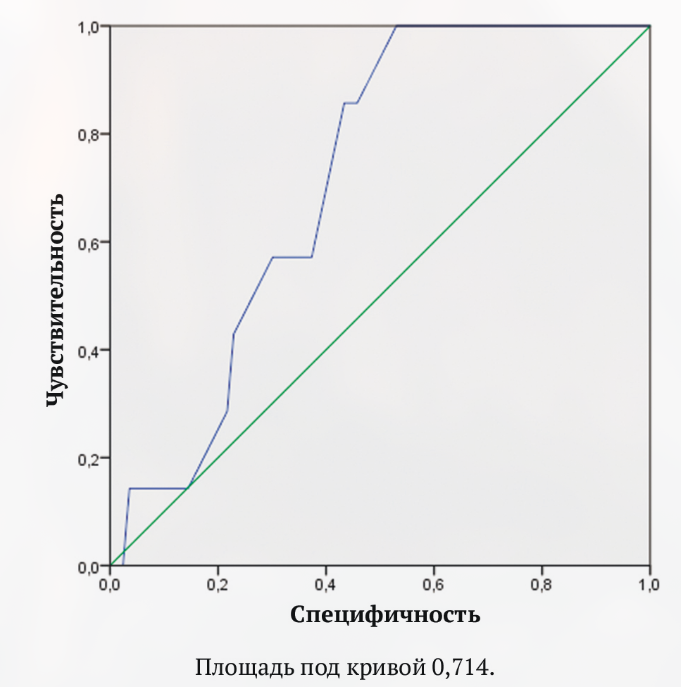
\includegraphics[width=0.5\linewidth]{fig1}
	\caption{ROC кривая. Логистическая регрессия. Предиктор возраст}
	\label{fig:roc}
\end{figure}

По результатам анализа ROC-кривой выявлена зависимость между предиктором возраст и регургитацией на митральном клапане, площадь под кривой говорит о среднем уровне взаимосвязи.

\begin{figure}[!ht]
\begin{tikzpicture}
	\begin{axis}[
		table/col sep = semicolon,
		height = 0.15\paperheight, 
		width = 0.3\paperwidth,
		xmin = 1927,
		xmax = 2014,
		/pgf/number format/1000 sep={}
		]
		
		\addplot table [x={Year}, y={Average population}] 
		{RussianDemography.csv};
	\end{axis}
\end{tikzpicture}
\end{figure}

\header{Заключение}

При малой выборке с небольшим количеством событий СИН имеют преимущество над другими методиками при определении предикторов влияния на зависимую переменную~\cite{Nosovski}.

ИНС позволяет нивелировать феномен разделения данных.

Необходимо более широко использовать методику в медицинской статистике.


\bigskip\bigskip\def\refname{\centerline{Список литературы}}


\bibliographystyle{ugost2008.bst}  %% стилевой файл для оформления по ГОСТу
\bibliography{cites}


\end{document}